% !TeX program = xelatex
% !BIB program = bibtex
\documentclass[type=bachelor]{suepthesis}
\SUEPSetup{
  cover = {date = 2026年6月},
  info = {
    title = 电力变压器故障诊断方法研究,
    titleEn = {A Study of Power Transformer Fault Diagnosis Methods},
    author = 张三,
    studentId = 20260001,
    supervisor = 李四教授,
    institution = 电气工程学院,
    major = 电气工程及其自动化,
    grade = 2022级,
    keywords = {电力变压器,故障诊断,气体分析},
    keywordsEn = {Power transformer,Fault diagnosis,Gas analysis}
  }
}
\usepackage{gbt7714}
\SUEPBibliographyStyle

\begin{document}
\MakeCover
\MakeOriginality
\frontmatter
\begin{abstract}
电力变压器的运行状态影响电力系统的可靠性。本文以变压器故障诊断为主题，介绍设备结构、故障分类及油中溶解气体分析的基本思路，讨论气体浓度变化与故障判断之间的联系。

本文通过图、表和公式展示诊断信息的组织方式，并给出相对产气速率的计算表达式。诊断过程需要结合设备运行记录、取样时间和试验条件，避免仅凭单一指标作出判断。

本示例用于演示论文结构与排版，正文和数据应在正式写作时替换为实际研究内容。
\end{abstract}

\begin{abstractEn}
The operating condition of power transformers affects the reliability of power systems. This example introduces transformer structure, fault classification, and the basic ideas of dissolved gas analysis. It discusses the relationship between changes in gas concentration and fault assessment.

Figures, tables, and equations illustrate how diagnostic information can be organized. The relative gas generation rate is presented as an example of a diagnostic indicator. Operating records, sampling intervals, and test conditions should be considered together.

This document demonstrates thesis structure and typesetting. Its text and data should be replaced with the author's actual research before submission.
\end{abstractEn}

\MakeTOC
\mainmatter
\chapter{引言}

\section{研究背景与意义}
电力变压器是电力系统的重要设备。随着设备容量和运行条件的变化，绝缘、冷却和保护装置的状态监测成为运行维护工作的重要组成部分。电机与电气设备的分析方法可参考相关文献\cite{gao1987}。

故障诊断需要将试验数据与设备结构、运行记录及维护经验结合起来。油中溶解气体分析为观察设备内部状态提供信息，但不同测量条件下的结果不能简单地直接比较。

\section{研究内容与论文结构}
本文介绍变压器的基本结构与故障分类，使用相对产气速率说明指标的计算方法，并通过图表展示诊断信息的整理方式。第二章给出方法与示例，第三章总结本文内容并讨论后续工作。

论文中的章、节编号和目录由模板自动生成。图表和公式通过交叉引用关联正文，修改顺序后无需手工重编号。

\chapter{电力变压器故障诊断方法}

\section{设备结构与诊断信息}
电力变压器由铁芯、绕组、油箱、绝缘套管、冷却装置和保护装置等组成。诊断信息包括设备参数、运行记录、试验结果和检修记录。图\ref{fig:data-management}展示历史示例中的数据管理界面，用于说明信息组织方式。

\begin{figure}[htbp]
  \centering
  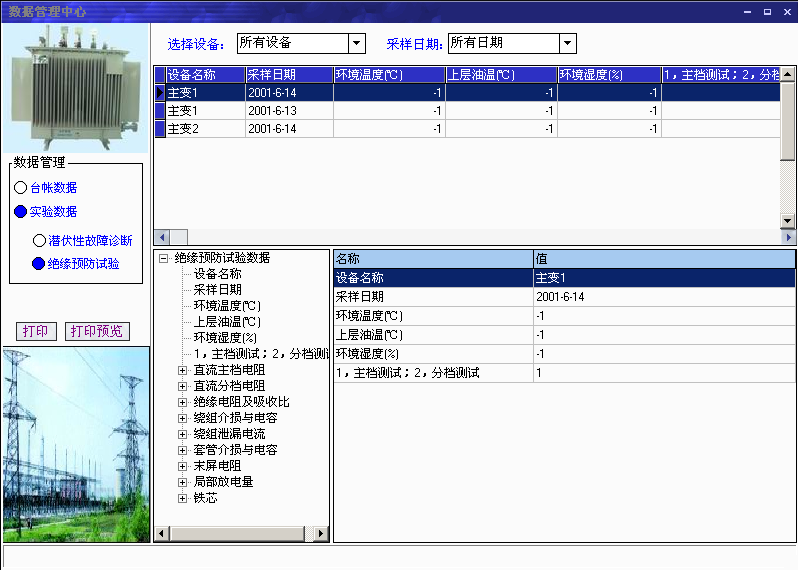
\includegraphics[width=0.85\linewidth]{images/data-management.png}
  \caption{数据管理界面示例}
  \label{fig:data-management}
\end{figure}

\section{故障分类与检测手段}
\subsection{故障分类}
故障可按发生部位划分为内部故障和外部故障。表\ref{tab:faults}列出用于说明分类方式的常见对象。实际分类还应结合具体设备和检测结果。

\begin{table}[htbp]
  \centering
  \caption{按发生部位划分的故障对象}
  \label{tab:faults}
  \begin{tabular}{p{0.42\linewidth}p{0.42\linewidth}}
    \toprule
    内部故障 & 外部故障 \\
    \midrule
    绕组绝缘、导线及连接部位 & 油箱与密封部件 \\
    铁芯及接地部位 & 冷却装置与控制设备 \\
    分接开关及引接线 & 绝缘套管与保护附件 \\
    \bottomrule
  \end{tabular}
\end{table}

\subsection{相对产气速率}
相对产气速率表示一定时间内气体浓度的相对变化，可写为
\begin{equation}
  \gamma_{\mathrm{r}} =
  \frac{C_{i,2}-C_{i,1}}{C_{i,1}}\frac{1}{\Delta t}\times 100\% .
  \label{eq:gas-rate}
\end{equation}

\begin{equationnotes}
  \item[$\gamma_{\mathrm{r}}$] 相对产气速率；
  \item[$C_{i,1}$] 第一次取样测得的第 $i$ 种气体浓度；
  \item[$C_{i,2}$] 第二次取样测得的第 $i$ 种气体浓度；
  \item[$\Delta t$] 两次取样之间的时间间隔。
\end{equationnotes}

式\eqref{eq:gas-rate}要求初始浓度非零，时间单位需保持一致。指标的解释还应考虑设备负荷、取样条件和测量误差。附录给出一组仅用于展示表格排版的数据。

\chapter{结论与展望}

\section{结论}
本文整理了变压器故障诊断所需的基本信息，介绍按发生部位分类的方式，并给出相对产气速率的计算表达式。诊断指标需要与设备结构、运行状态和试验条件结合使用。

\section{后续工作}
后续研究可收集不同工况下的实际数据，分析测量误差对指标的影响，并比较不同诊断方法的适用条件。正式论文应在此处总结自己的研究结果和局限。


\backmatter
\begin{acknowledgements}
感谢指导教师和同学在研究与论文写作过程中给予的帮助。
\end{acknowledgements}

\begin{bibprint}
  \bibliography{references}
\end{bibprint}

\begin{appendices}
\chapter{诊断数据示例}
以下数据取自历史样张，仅用于展示表格排版，并非本文的实测结果。正式论文应填写自己的数据及单位、来源与试验条件。

\begin{table}[htbp]
  \centering
  \caption{气体分析数据示例}
  \begin{tabular}{lr}
    \toprule
    气体 & 浓度（$\mu\mathrm{L}/\mathrm{L}$） \\
    \midrule
    $\mathrm{H}_2$ & 77.5 \\
    $\mathrm{CH}_4$ & 189.6 \\
    $\mathrm{C}_2\mathrm{H}_6$ & 81.2 \\
    $\mathrm{C}_2\mathrm{H}_4$ & 329 \\
    $\mathrm{C}_2\mathrm{H}_2$ & 2.4 \\
    $\mathrm{CO}$ & 151 \\
    $\mathrm{CO}_2$ & 18991 \\
    \bottomrule
  \end{tabular}
\end{table}
\end{appendices}

\end{document}
